\scanpage{71}
\mspage{\deleted{\unsure{69|79}}\unsure{70|79}}

Il revient au $=$ de dire que $F$ et $F'$ ont $=$ cosupport, ou encore, même support.

\unsure{Donnons nous} un support.

% G1 margin-mark columns: the two disconnected groups are drawn, without assigning them a linguistic function.
\figure{

\begin{tikzpicture}[x=1cm,y=1cm]
  \node[anchor=north west,align=left] at (2.15,0.55) {Une autre façon de dire que $F,G\ \text{disj.}$\\[0.35em]
  $\Longrightarrow F',G\ \text{disj}$, est ainsi :};
  \fill (0.10,0.02) ellipse (0.016 and 0.024);
  \draw[line width=0.8pt] (0.10,-0.04)--(0.11,-0.10)--(0.10,-0.16);
  \fill (0.10,-0.20) circle (0.014);
  \draw[line width=0.8pt] (0.10,-0.24)--(0.11,-0.29)--(0.10,-0.35);
  \fill (0.17,-0.40) circle (0.018);
  \fill (1.88,0.30) circle (0.013);
  \draw[line width=0.7pt] (1.87,0.26)--(1.88,0.21);
  \fill (1.89,0.15) circle (0.015);
  \fill (1.89,0.09) circle (0.013);
  \fill (1.87,-0.03) circle (0.017);
\end{tikzpicture}}

% G2: the long rising stroke crosses de beneath the raised addition; deletion versus a crossing insertion arm remains uncertain.
\figure{
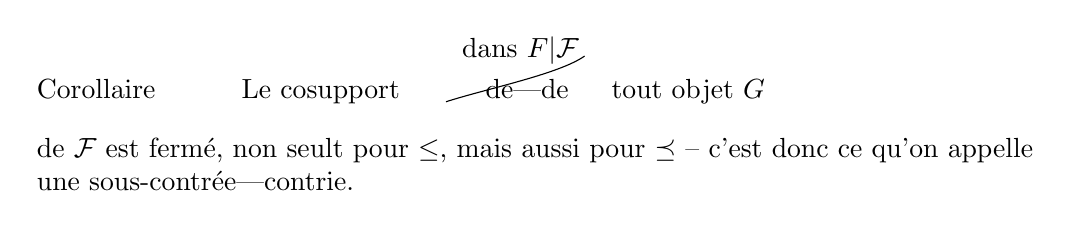
\begin{tikzpicture}[x=1cm,y=1cm]
  \node[anchor=base west] at (0,0) {\uline{Corollaire}};
  \node[anchor=base west] at (2.60,0) {Le cosupport};
  \node[anchor=base west] at (5.70,0) {\unsure{\deleted{de}|de}};
  \node[anchor=base west] at (5.40,0.52) {\inserted{dans $\unsure{F|\mathcal F}$}};
  \draw (5.32,-0.04) .. controls (5.85,0.13) and (6.75,0.31) .. (7.08,0.54);
  \node[anchor=base west] at (7.30,0) {tout objet $G$};
  \node[anchor=north west,text width=12.7cm,align=left] at (0,-0.38) {de $\mathcal F$ est fermé, non seult pour $\leq$, mais aussi pour $\preceq$ -- c'est donc ce qu'on appelle une \uline{sous}-\unsure{contrée|contrie}.};
\end{tikzpicture}}

% G3 itou high mark: the final detached high stroke is reproduced; its role in the word is uncertain.
\figure{

\begin{tikzpicture}[x=1cm,y=1cm]
  \node[anchor=base west] at (0,0) {Donc};
  \node[anchor=base west] at (1.15,0) {\unsure{itou}};
  \draw (1.91,0.33)--(1.96,0.49)--(2.03,0.38);
  \node[anchor=base west] at (3.45,0) {pour toute partie $\Phi\subset\mathcal F$.};
\end{tikzpicture}}

% G4 right punctuation: the punctuation after leq is drawn in place. The loop and short right arm meet the sheet edge.
\figure{
\begin{tikzpicture}[x=1cm,y=1cm]
  \node[anchor=base west] at (0,0) {En d'autres termes, \deleted{toute} partie};
  \node[anchor=base west] at (0,-0.58) {de $\mathcal F$ qui est un $\mathcal F$-support (ou};
  \node[anchor=base west] at (0,-1.16) {``$\mathcal F$-\unsure{saturee|saturée}, sous-entendu : en termes de $\leq$};
  \node[anchor=base west] at (12.05,-1.16) {\unsure{\begin{tikzpicture}[x=1cm,y=1cm,baseline=0pt]
    \draw[line width=0.6pt] (0.04,0.01) .. controls (0.09,-0.09) and (0.04,-0.17) .. (-0.02,-0.20);
    \draw (0.16,0.36) .. controls (0.43,0.10) and (0.43,-0.10) .. (0.23,-0.23);
    \draw (0.30,0.22) .. controls (0.33,0.26) and (0.38,0.18) .. (0.45,0.17) .. controls (0.54,0.15) and (0.41,0.08) .. (0.35,0.04);
    \draw (0.37,0.02)--(0.54,-0.02);
  \end{tikzpicture}}};
  \node[anchor=base west] at (0,-1.85) {cf \unsure{pg|page|pge} $67$) est \unsure{automatiquemt|automatiquement} \deleted{\unsure{f}}une};
  \node[anchor=base west] at (0,-2.43) {sous-contrée.};
\end{tikzpicture}}

% The following two-position folio and draft are upside down on the sheet.
% The second numeral is overwritten; the broad cancellation strokes start below the folio.
\mspage{5\rlap{\deleted{\unsure{4|3}}}5}

% G5 inverted cancelled draft. Text occurs once, in the same group as the boundary and oblique cancellation strokes.
% The isolated glyph under the first Phi is not securely separable from its retracing.
\figure{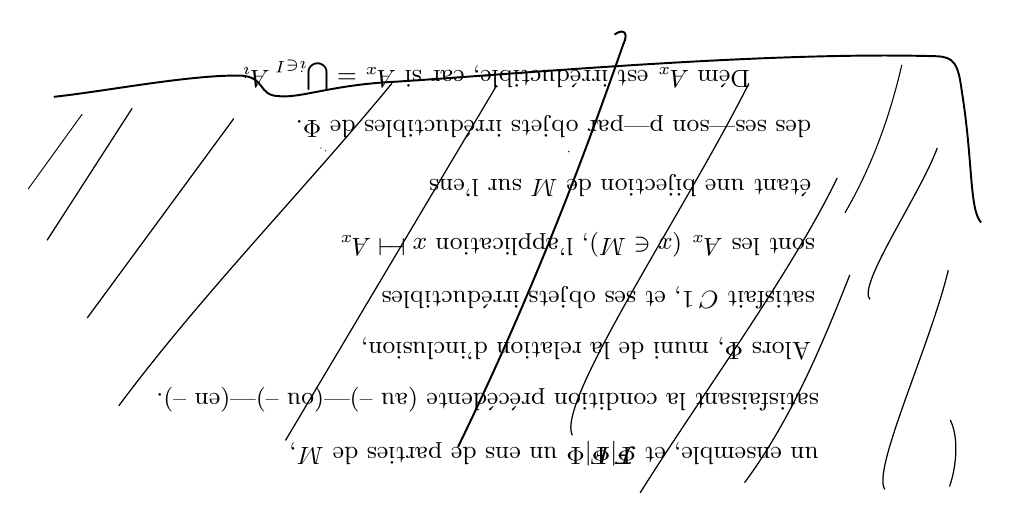
\begin{tikzpicture}[x=0.005cm,y=-0.005cm,font=\small]
\begin{scope}[rotate=180,transform shape]
\node[anchor=base west,inner sep=0pt] at (410,220) {\deleted{un ensemble, et $\unsure{\rlap{\ensuremath{\deleted{\mathcal F}}}\Phi|\rlap{\ensuremath{\deleted{F}}}\Phi|\Phi}$ un ens de parties de $M$,}};
\node[anchor=base west,inner sep=0pt] at (410,355) {\deleted{satisfaisant la condition précédente \unsure{(au --)|(ou --)|(en --)}.}};
\node[anchor=base west,inner sep=0pt] at (430,485) {\deleted{Alors $\Phi$, muni de la relation d'inclusion,}};
\node[anchor=base west,inner sep=0pt] at (420,615) {\deleted{satisfait $C\,1$, et ses objets irréductibles}};
\node[anchor=base west,inner sep=0pt] at (420,750) {\deleted{sont les $A_x$ $(x\in M)$, l'application $x\mathrel{\vdash\joinrel\dashv} A_x$}};
\node[anchor=base west,inner sep=0pt] at (430,900) {\deleted{étant une bijection de $M$ sur l'ens}};
\node[anchor=base west,inner sep=0pt] at (430,1050) {\deleted{des \deleted{\unsure{ses|son}} \deleted{\unsure{p|par}} objets irréductibles de $\Phi$.}};
\node[anchor=base west,inner sep=0pt] at (585,1177) {\deleted{Dém $A_x$ est irréductible, car si $A_x=\bigcup_{i\in I} A_i$}};
% One detached high point after the second inner cancellation, and two low points beneath irreductibles.
\fill (1046,970) circle (2.0);
\fill (1663,972) circle (1.7);
\fill (1675,979) circle (1.7);
% The boundary is open at the scan edge; its upper continuation is not inferred.
\draw[line width=0.7pt] (0,790) .. controls (30,825) and (20,945) .. (49,1125)
 .. controls (58,1195) and (70,1210) .. (112,1212)
 .. controls (550,1225) and (1200,1165) .. (1492,1147)
 .. controls (1650,1139) and (1730,1104) .. (1784,1111)
 .. controls (1835,1113) and (1815,1159) .. (1878,1163)
 .. controls (2010,1165) and (2215,1124) .. (2353,1109);
% Thirteen distinct oblique or curved cancellation strokes.
\draw[line width=0.45pt] (80,120) .. controls (62,170) and (56,245) .. (78,289);
\draw[line width=0.45pt] (244,113) .. controls (278,160) and (130,475) .. (83,669);
\draw[line width=0.45pt] (282,595) .. controls (315,630) and (155,860) .. (111,979);
\draw[line width=0.45pt] (600,130) .. controls (485,285) and (405,474) .. (333,657);
\draw[line width=0.45pt] (865,104) .. controls (720,336) and (480,664) .. (365,903);
\draw[line width=0.40pt] (345,815) .. controls (276,934) and (231,1060) .. (201,1190);
\draw[line width=0.45pt] (1037,250) .. controls (1080,332) and (758,808) .. (589,1143);
\draw[line width=0.72pt] (1327,221) .. controls (1130,625) and (993,997) .. (908,1242)
 .. controls (892,1275) and (910,1282) .. (930,1267);
\draw[line width=0.45pt] (1765,237) -- (1229,1138);
\draw[line width=0.45pt] (2188,325) .. controls (1978,607) and (1714,877) .. (1495,1143);
\draw[line width=0.45pt] (2268,548) -- (1896,1054);
\draw[line width=0.45pt] (2370,745) -- (2154,1080);
\draw[line width=0.35pt] (2418,875) -- (2281,1065);
\end{scope}
\end{tikzpicture}}
